\documentclass[10pt]{article}
\usepackage{graphicx}
\usepackage{amssymb}
\usepackage[fleqn]{amsmath}
\usepackage{nccmath}
\usepackage{cases}
\usepackage{hyperref}
\usepackage{multicol}
\usepackage{tikz}
\usepackage{pgfplots}
\usepackage{enumitem}
\usepackage{pdfpages}
\pgfplotsset{compat=1.18}
\usepackage{float}
\DeclareMathOperator*{\argmin}{arg\,min}

\title{\bf Math 164: Problem Set 4}
\date{2/2/2024}
\author{\bf Owen Jones}
\begin{document}
\maketitle
\begin{enumerate}
    \item [\textbf{6.18}] Let $\tilde{x}=\underset{x\in \mathbb{R}}{\argmin}f(x)$ where $f(x)=\displaystyle\sum_{i=1}^{n}{(x_i-x)}^2$. 
    By the FONC, $f'(\tilde{x})=0\Rightarrow \displaystyle2\sum_{i=1}^{n}{(x_i-\tilde{x})}=0$. Thus, $\tilde{x}=\frac{1}{n}\displaystyle\sum_{i=1}^{n}x_i$
    \item [\textbf{6.21}] \begin{enumerate}
        \item Let $\mathbf{x}^*=\underset{x\in \mathbb{R}}{\argmin}f(x)$ where $f(x)=\frac{\sqrt{1+x^2}}{v_1}+\frac{\sqrt{1+{(d-x)}^2}}{v_2}$.\\
        By the FONC, $f'(\mathbf{x}^*)=0\Rightarrow f'(\mathbf{x}^*)=\frac{\mathbf{x}^*}{\sqrt{1+{\mathbf{x}^*}^2}v_1}-\frac{d-\mathbf{x}^*}{\sqrt{1+{(d-\mathbf{x}^*)}^2}v_2}=0\\
        \Rightarrow \frac{\mathbf{x}^*}{\sqrt{1+{\mathbf{x}^*}^2}v_1}=\frac{d-\mathbf{x}^*}{\sqrt{1+{(d-\mathbf{x}^*)}^2}v_2}\\
        \Rightarrow \frac{v_1}{v_2}=\frac{\frac{\mathbf{x}^*}{\sqrt{1+{\mathbf{x}^*}^2}}}{\frac{d-\mathbf{x}^*}{\sqrt{1+{(d-\mathbf{x}^*)}^2}}}=\frac{\sin{\theta_1}}{\sin{\theta_2}}$.
        \item $f''(x)=\frac{1}{{(1+x^2)}^\frac{3}{2}v_1}+\frac{1}{{(1+{(d-x)}^2)}^\frac{3}{2}v_2}$. Because $f''(x)>0$ for all $x$, the SOSC is satisfied.
    \end{enumerate}
    \item [\textbf{6.25}] Suppose $\mathbf{d}$ is a feasible direction at $\mathbf{x}\in\mathbf{\Omega}$. 
    It follows, there exists some $\alpha_0>0$ s.t $\forall\alpha\in[0,\alpha_0]$ $\mathbf{x}+\alpha\mathbf{d}\in\mathbf{\Omega}$.
    Therefore $\mathbf{A}(\mathbf{x}+\alpha\mathbf{d})=\mathbf{A}\mathbf{x}+\alpha\mathbf{A}\mathbf{d}=\mathbf{b}+\alpha\mathbf{A}\mathbf{d}=\mathbf{b}\\
    \Rightarrow \mathbf{A}\mathbf{d}=\mathbf{0}$.\\
    Suppose $\mathbf{A}\mathbf{d}=\mathbf{0}$.
    Let $\mathbf{x}\in\mathbf{\Omega}$, and let $\alpha>0$.
    It follows $\mathbf{A}(\mathbf{x}+\alpha\mathbf{d})=\mathbf{A}\mathbf{x}+\alpha\mathbf{A}\mathbf{d}=\mathbf{b}+\alpha\cdot\mathbf{0}=\mathbf{b}$.
    Thus, $\mathbf{d}$ is a feasible direction at $\mathbf{x}\in\mathbf{\Omega}$.
    \item [\textbf{6.26}] Since $\mathbf{0}$ is a boundary point, we need to show there exists some feasible direction $\mathbf{d}$ s.t $\mathbf{d}\nabla f(\mathbf{0})<\mathbf{0}$.
    $\mathbf{d}={[1,1]}^{\top}$ is clearly a feasible direction because both components are greater than $0$. 
    Because $f(\mathbf{0})\neq \mathbf{0}$, $\frac{\partial f}{\partial x_1}(\mathbf{0})\le 0$, and $\frac{\partial f}{\partial x_2}(\mathbf{0})\le 0$, at least one of $\frac{\partial f}{\partial x_1}(\mathbf{0})<0$ or $\frac{\partial f}{\partial x_2}(\mathbf{0})<0$ must be true.
    Thus, $\mathbf{d}\nabla f(\mathbf{0})=\frac{\partial f}{\partial x_1}(\mathbf{0})+\frac{\partial f}{\partial x_2}(\mathbf{0})<0$.
    Hence, $f(\mathbf{0})$ cannot be a local minimizer because it doesn't satisfy the FONC.
    \item [\textbf{6.27}] Because $f(\mathbf{x})=\mathbf{c}^\top\mathbf{x}\Rightarrow \nabla f(\mathbf{x})=\mathbf{c}\neq \mathbf{0}$. 
    Thus, for any interior point, $\nabla f(\mathbf{x})\neq \mathbf{0}$, so there can't be any interior points that satisfy the FONC.
    Hence, if there exists a local minimizer over the set $\mathbf{\Omega}$, it must lie on the boundary of $\mathbf{\Omega}$
    \item [\textbf{7.2(d)}] $f'(x)=2x-4\sin(x),f''(x)=2-4\cos(x) \Rightarrow x^{(k+1)}=x^{(k)}-\frac{x-2\sin(x)}{1-2\cos(x)}$ gives us our formula for Newton's Method.\\
    $x^{(0)}=1,\quad x^{(1)}=-7.47274,\quad x^{(2)}=14.47852,\quad x^{(3)}=6.93511$
    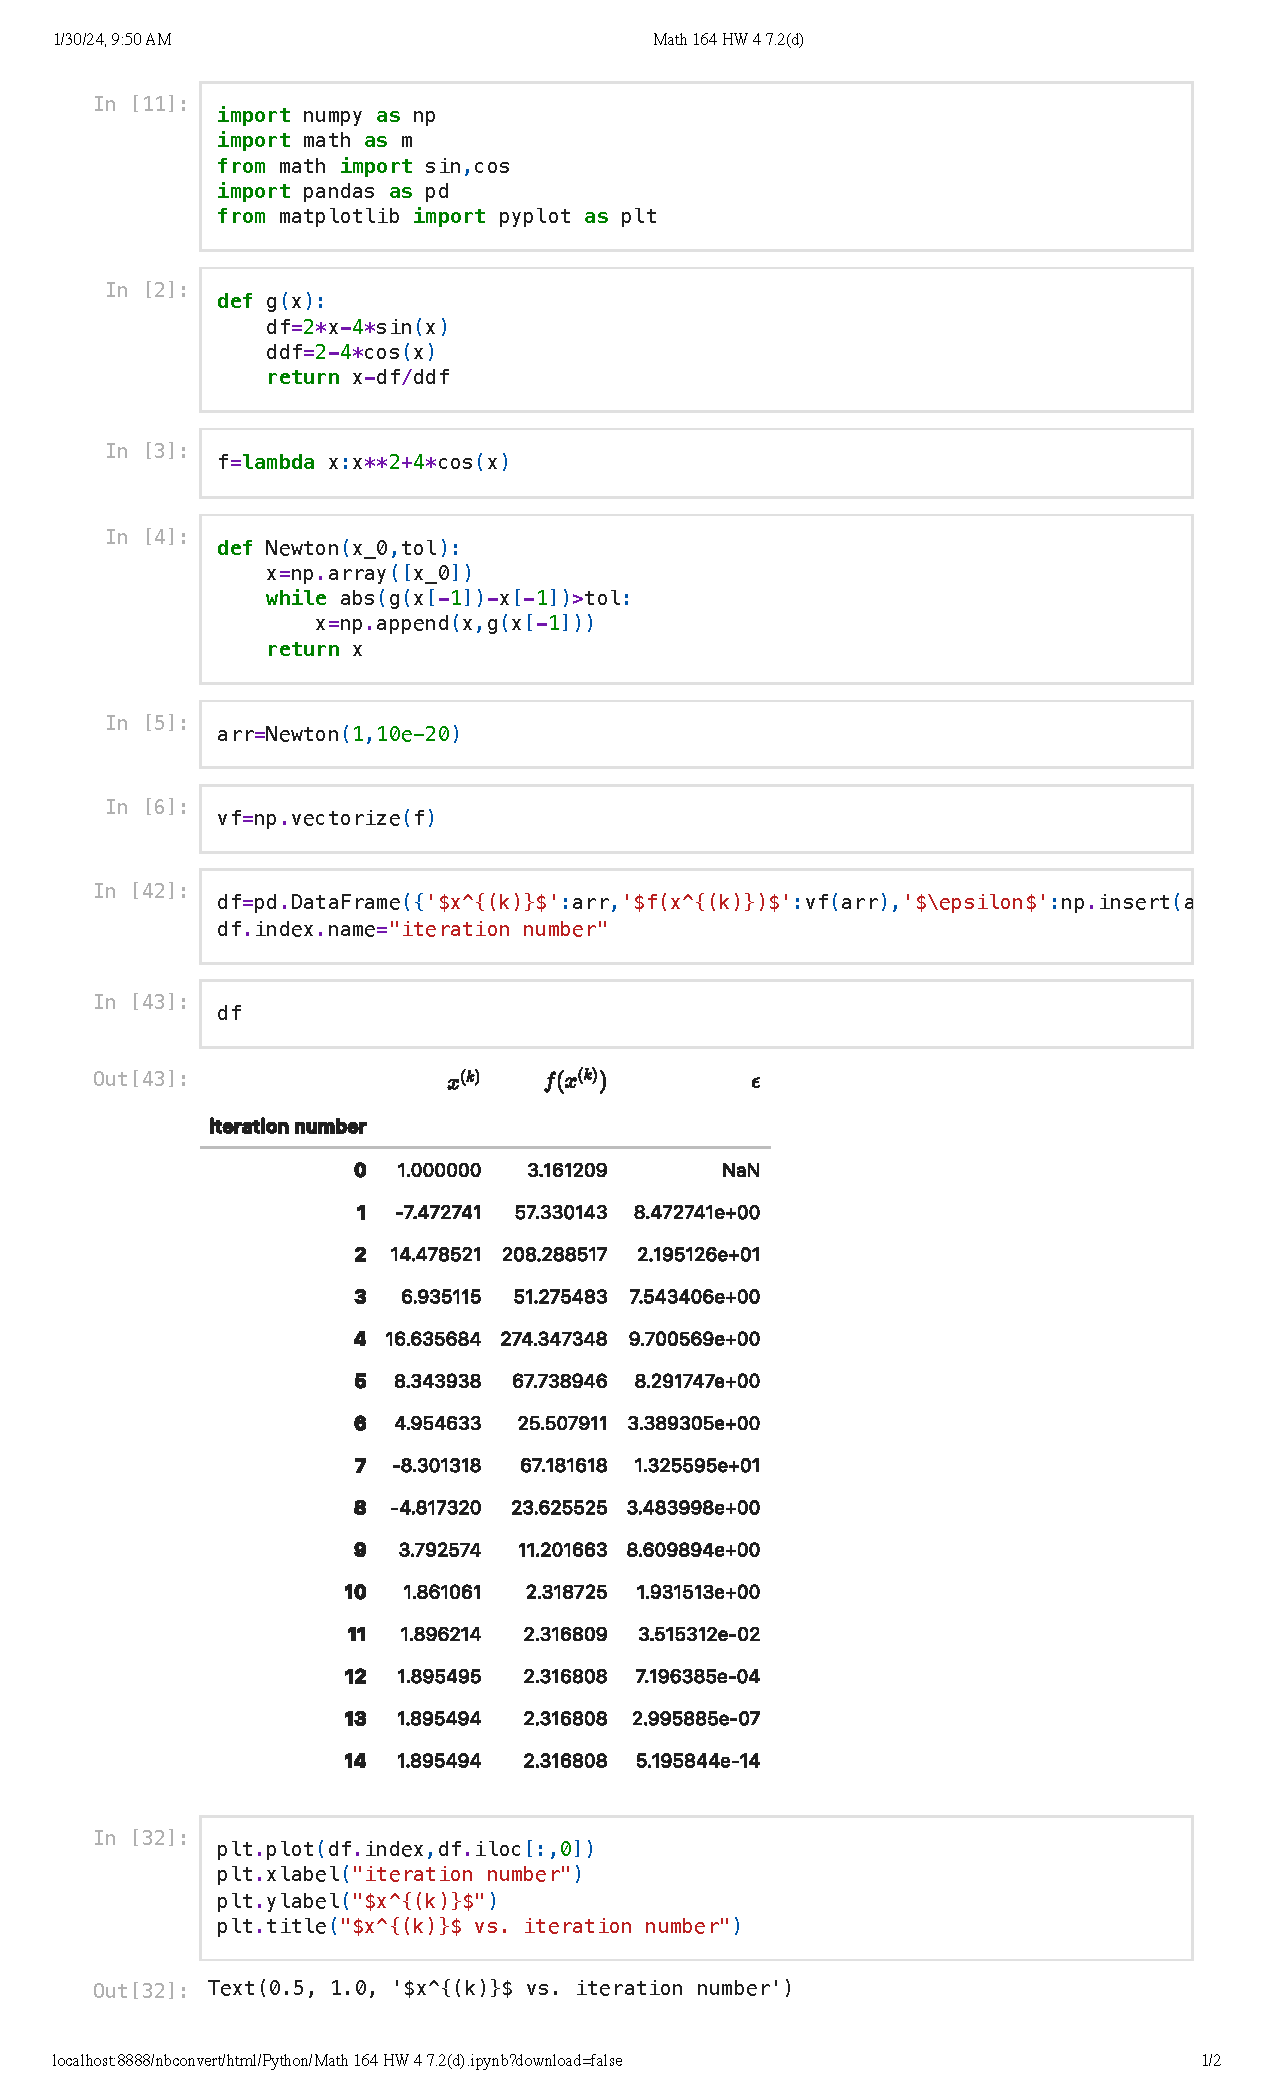
\includepdf[pages=-]{Math 164 HW 4 7.2(d).pdf}
\end{enumerate}
\end{document}